\chapter{Modeling} 

\section{Background}

\subsection{Model architecture} 

The Transformer architecture, introduced by Vaswani et al. in 2017 \cite{vaswani2017attention}, has become a pivotal model in natural language processing tasks.

\hfill \break
\textbf{Encoder:} \\
The Encoder processes an input sequence using multi-head self-attention and position-wise feed-forward networks.


\begin{itemize}
    \item \textbf{Multi-Head Self-Attention:} This mechanism allows each word in the input sequence to attend to all other words simultaneously, capturing dependencies and relationships effectively.
    
    \item \textbf{Position-wise Feed-Forward Networks:} After attention computation, a position-wise fully connected feed-forward network is applied independently to each position.
\end{itemize}

\begin{figure}[h!]
	\centering
	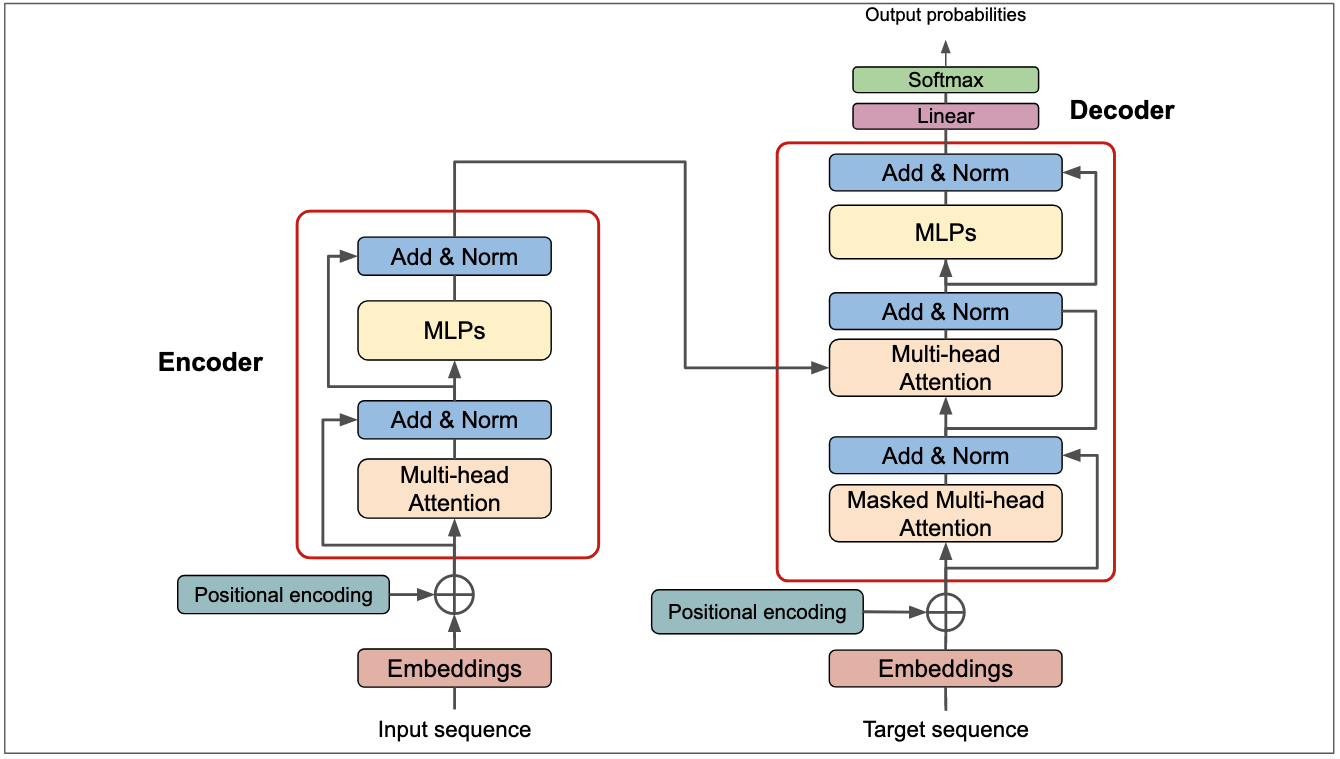
\includegraphics[scale=0.3]{figures/transformer.png}
	\caption{Transformer Architecture}
\end{figure}

\hfill \break
\textbf{Decoder:}  \\
The Decoder generates an output sequence by attending to the Encoder's output and performing masked self-attention and cross-attention over the input sequence.


\begin{itemize}
    \item \textbf{Masked Multi-Head Self-Attention:} During training, masking is applied to prevent future positions from being used, allowing each word to attend only to previous positions.
    
    \item \textbf{Multi-Head Cross-Attention:} This sub-layer attends to the encoded input sequence, helping the decoder focus on relevant parts of the input sequence when generating each word in the output sequence.
    
    \item \textbf{Position-wise Feed-Forward Networks:} A position-wise fully connected feed-forward network is applied to each position after attention computation.
\end{itemize}


\hfill \break
\textbf{Key Innovations:}

\begin{itemize}
    \item \textbf{Self-Attention Mechanism:} Enables capturing dependencies across the entire input sequence.
    
    \item \textbf{Positional Encoding:} Provides information about the order of tokens in input sequences.
    
    \item \textbf{Residual Connections and Layer Normalization:} Address vanishing gradient problem and improve convergence speed in deep models.
\end{itemize}

\newpage


\subsection{LLMs}

\hfill \break
\textbf{ (LLMs)} \\

LLMs such as GPT (Generative Pre-trained Transformer) are pivotal in natural language processing. These models are trained on large-scale datasets using unsupervised learning techniques before fine-tuning on specific tasks.

\hfill \break
\textbf{Training Process:} \\

LLMs are typically pre-trained using a variant of the Transformer architecture. The training process involves:

\begin{itemize}
    \item \textbf{Pre-training on Large Corpora:} LLMs are trained on vast amounts of text data to learn general language patterns and representations. This phase helps the model capture semantic relationships and syntactic structures.
    
    \item \textbf{Objective Functions:} During pre-training, objectives like language modeling (predicting the next word in a sequence) and masked language modeling (predicting masked-out words) are used to teach the model about language coherence and context understanding.
    
    \item \textbf{Fine-tuning:} After pre-training, LLMs can be fine-tuned on smaller, task-specific datasets to adapt to specific applications such as question answering, summarization, or language translation.
\end{itemize}

\hfill \break
\textbf{Key Details:} \\

LLMs leverage the Transformer's self-attention mechanism, allowing them to process and generate text while considering global dependencies efficiently. Key aspects include:

\begin{itemize}
    \item \textbf{Self-Attention:} Enables the model to weigh the significance of each word in the context of the entire input sequence.
    
    \item \textbf{Positional Encodings:} Provides information about the order of tokens in input sequences, compensating for the lack of sequential information in the Transformer's architecture.
    
    \item \textbf{Fine-grained Representations:} LLMs produce contextual embeddings that capture intricate linguistic nuances, making them versatile for various natural language processing tasks.
\end{itemize}

\begin{figure}[h!]
	\centering
	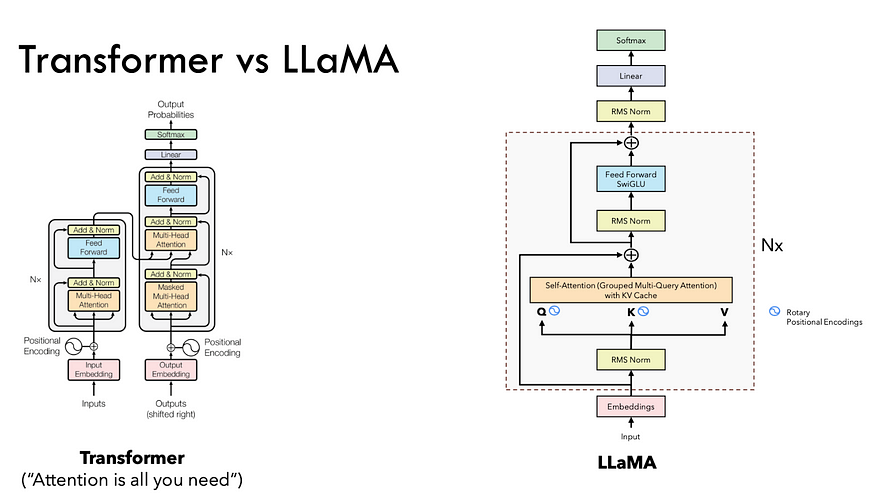
\includegraphics[scale=0.5]{figures/llama.png}
	\caption{Transformer vs LLAMA }
\end{figure}

\hfill \break
\textbf{Challenges of Training Large Language Models (LLMs)}

Training Large Language Models (LLMs) such as GPT (Generative Pre-trained Transformer) poses several challenges due to the scale and complexity of the models involved:

\begin{itemize}
    \item \textbf{Computational Resources:} LLMs require substantial computational resources, including high-performance GPUs or TPUs, to handle the massive amounts of data and computations involved in training.
    
    \item \textbf{Data Efficiency:} Despite their size, LLMs still require vast amounts of labeled or unlabeled data for effective training. Acquiring and preprocessing such large datasets can be challenging.
    
    \item \textbf{Training Time:} Training LLMs is time-consuming, often taking days or even weeks on powerful hardware. This extended duration can hinder rapid experimentation and model iteration.
    
    \item \textbf{Fine-tuning Challenges:} While pre-training is effective, fine-tuning LLMs for specific tasks requires careful tuning of hyperparameters and regularization techniques to prevent overfitting and ensure optimal performance.
    
    \item \textbf{Memory and Scalability:} Managing memory usage and ensuring scalability across distributed systems are critical challenges, especially as models grow larger and more complex.
    
    \item \textbf{Ethical Considerations:} The sheer size and capability of LLMs raise ethical concerns related to bias, fairness, and the potential misuse of generated content.
\end{itemize}

\begin{figure}[h!]
	\centering
	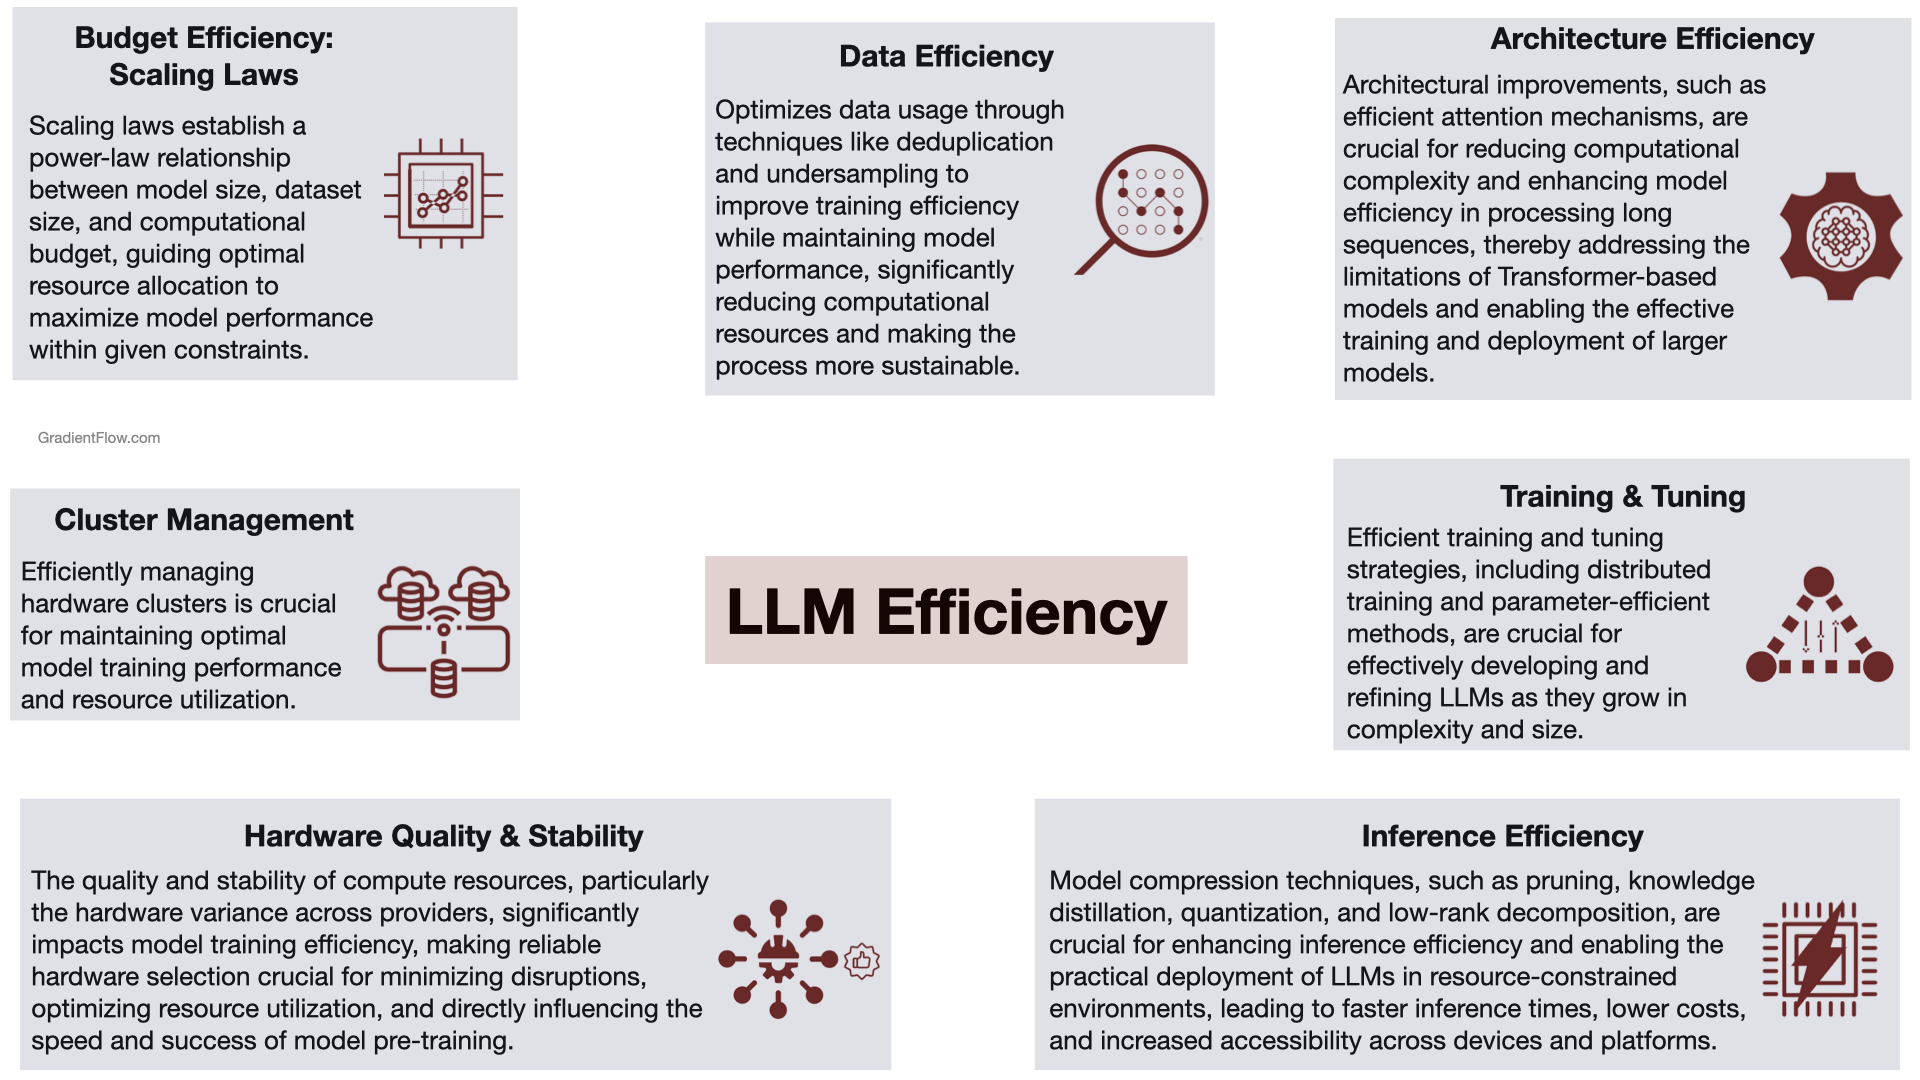
\includegraphics[scale=0.2]{figures/llm computational resources.jpeg}
	\caption{challenges of training LLMs }
\end{figure}
\newpage

\subsection{Instruction Fine-tuning} 

\hfill \break
\textbf{What is instruction tuning?} \\

\hfill \break
Instruction tuning is a subset of the broader category of fine-tuning techniques used to adapt pre-trained foundation models for downstream tasks. Foundation models can be fine-tuned for a variety of purposes, from style customization to supplementing the core knowledge and vocabulary of the pre-trained model to optimizing performance for a specific use case. Though fine-tuning is not exclusive to any specific domain or artificial intelligence model architecture, it has become an integral part of the LLM lifecycle. For example, Meta’s Llama 2 model family is offered (in multiple sizes) as a base model, as a variant fine-tuned for dialogue (Llama-2-chat) and as a variant fine-tuned for coding (Code Llama).


\hfill \break
Instruction tuning is not mutually exclusive with other fine-tuning techniques. For example, chat models often undergo both instruction tuning and reinforcement learning from human feedback (RLHF), a fine-tuning technique that aims to improve abstract qualities like helpfulness and honesty; models fine-tuned for coding often undergo both instruction tuning (to broadly optimize responses for instruction following) and additional fine-tuning on programming-specific data (to augment the model’s knowledge of coding syntax and vocabulary).

\hfill \break
\textbf{Why instruction tune LLMs?} \\
\hfill \break
The pre-training process for autoregressive language models—LLMs used for generating text, like Meta’s Llama 2, OpenAI’s GPT, Google’s Gemini or IBM’s Granite—optimizes these LLMs to simply predict the next word(s) in a given sequence until it’s complete.

\hfill \break
LLMs are pre-trained using self-supervised learning on a massive corpus of written content. In pre-training, autoregressive models are provided the beginning of a text sample and repeatedly tasked with predicting the next word in the sequence until the end of the excerpt. For each prediction, the actual next word of the original sample sentence serves as “ground truth.” Through optimization algorithms like gradient descent that iteratively adjust model parameters—the varying weights and biases applied to the mathematical operations occurring at each node in a neural network—in a way that brings the model’s predictions closer to the original text, the model “learns” the linguistic patterns in its training data (and, by extension, the “knowledge” conveyed in those linguistic patterns).

\hfill \break
\textbf{Example of instruction promote} \\

\begin{center}
\begin{figure}[h!]
\centering
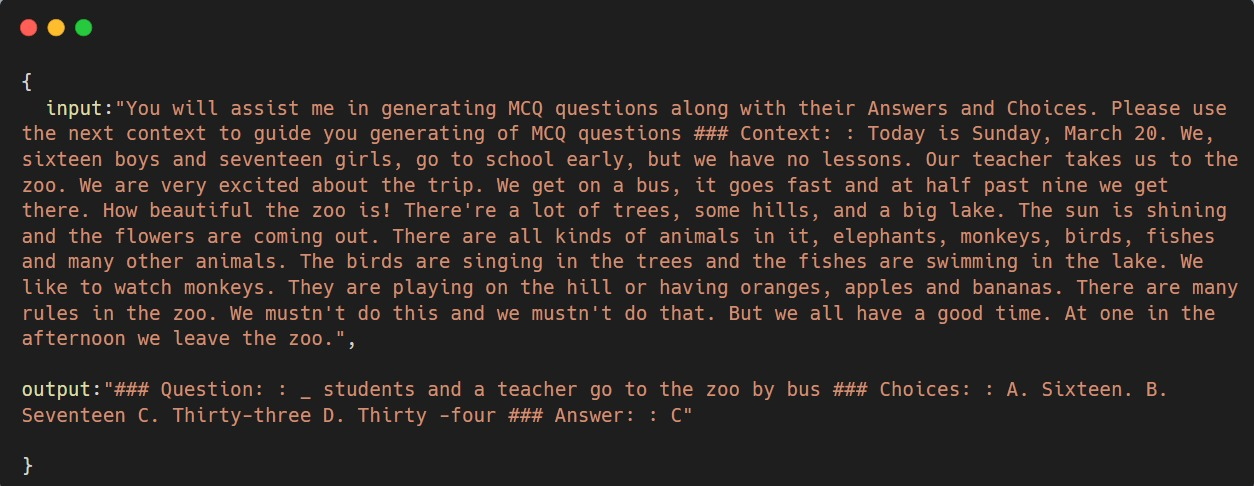
\includegraphics[scale=0.5,width=20.75cm,height=10cm, center]{figures/instruction dataset.png}
\caption{ Example of instruction promote }
\end{figure}
\end{center}

\hfill \break
Here is the link to the Dataset repository: \url{https://huggingface.co/datasets/shredder-31/QG_QusestionsData}


\newpage
\subsection{QLORA: Efficient Finetuning of Quantized LLMs} 

\hfill \break
\textbf{QLORA: Efficient Finetuning of Quantized LLMs}

\hfill \break
``QLORA: Efficient Finetuning of Quantized LLMs'' \cite{dettmers2024qlora} is a research paper that focuses on optimizing the fine-tuning process for quantized large language models (LLMs). Here’s a detailed explanation of the key concepts and contributions of QLORA:


\hfill \break
Large Language Models (LLMs) like GPT (Generative Pre-trained Transformer) have achieved significant success in various natural language processing (NLP) tasks. However, these models are computationally intensive and memory-intensive, making them challenging to deploy in resource-constrained environments like mobile devices or edge computing platforms.

\hfill \break
Quantization is a technique used to address these challenges. It involves reducing the precision of model parameters (e.g., from 32-bit floating point to 8-bit integers) to reduce memory usage and improve inference speed. However, quantization often leads to a drop in performance unless the model is fine-tuned properly.

\hfill \break
\textbf{Key Challenges Addressed by QLORA}

\hfill \break
1. \textbf{Efficient Fine-tuning}: Fine-tuning a quantized LLM involves adjusting the model weights to perform well on a specific downstream task while maintaining the benefits of quantization. This process is crucial because quantization can degrade model accuracy if not managed properly.

\hfill \break
2. \textbf{Optimal Hyperparameter Search}: Finding the right hyperparameters (e.g., learning rate, batch size) for fine-tuning quantized models is non-trivial due to the interaction between quantization and model training dynamics.

\hfill \break
\textbf{Contributions of QLORA}

QLORA proposes several techniques to improve the efficiency and effectiveness of fine-tuning quantized LLMs:


\hfill \break
1. \textbf{Layer-wise Quantization-aware Optimization}: QLORA introduces a method to optimize the learning rate and weight decay for each layer of the quantized model separately. This approach accounts for the different sensitivities of layers to quantization errors, improving overall performance.


\hfill \break
2. \textbf{Dynamic Range Scaling}: QLORA employs dynamic range scaling during fine-tuning, which adjusts the quantization parameters (such as scale and zero-point) based on the statistics of the input data. This adaptive scaling helps mitigate the impact of quantization on model accuracy.


\hfill \break
3. \textbf{Efficient Search for Hyperparameters}: QLORA incorporates techniques for efficiently searching the hyperparameter space, such as Bayesian optimization or grid search tailored for quantized models. This ensures that the fine-tuning process is both effective and resource-efficient.

\begin{figure}[h!]
	\centering
	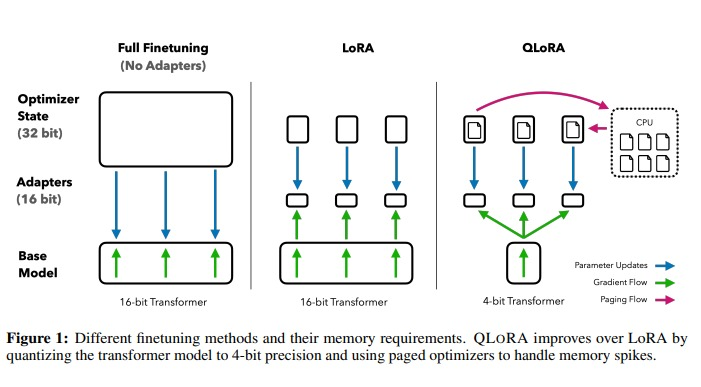
\includegraphics[scale=0.5]{figures/Qlora.jpeg}
	\caption{ Qlora }
\end{figure}
\newpage
\subsection{RAG: Retrieval-Augmented Generation for Knowledge-Intensive NLP Tasks}


Retrieval-Augmented Generation (RAG) represents a significant advancement in natural language processing \cite{lewis2020retrieval}, particularly for knowledge-intensive tasks. This approach integrates both retrieval-based and generation-based models to leverage external knowledge sources effectively. 

The workflow of Retrieval-Augmented Generation typically involves the following steps:
\begin{itemize}
    \item \textbf{Retrieval Phase:}
    \begin{itemize}
        \item \textit{Query Formation:} The input query or prompt is formulated.
        \item \textit{Retrieval:} A retrieval model searches through external knowledge sources (like Wikipedia, databases, or custom corpora) to extract relevant passages or documents related to the query.
    \end{itemize}
    \item \textbf{Integration Phase:}
    \begin{itemize}
        \item \textit{Candidate Selection:} The retrieved documents or passages are filtered to select the most relevant ones based on similarity metrics or other criteria.
        \item \textit{Context Integration:} The selected documents are integrated into the context of the generation model. This can involve concatenating retrieved text with the original input or dynamically attending to relevant parts during generation.
    \end{itemize}
    \item \textbf{Generation Phase:}
    \begin{itemize}
        \item \textit{Text Generation:} The integrated context is fed into a generation model (often a transformer-based model) to produce a coherent and contextually relevant output.
        \item \textit{Fine-Tuning:} The model may be fine-tuned on task-specific data to improve performance on particular NLP tasks, ensuring the generated outputs are accurate and contextually appropriate.
    \end{itemize}
\end{itemize}

\begin{figure}[h!]
	\centering
	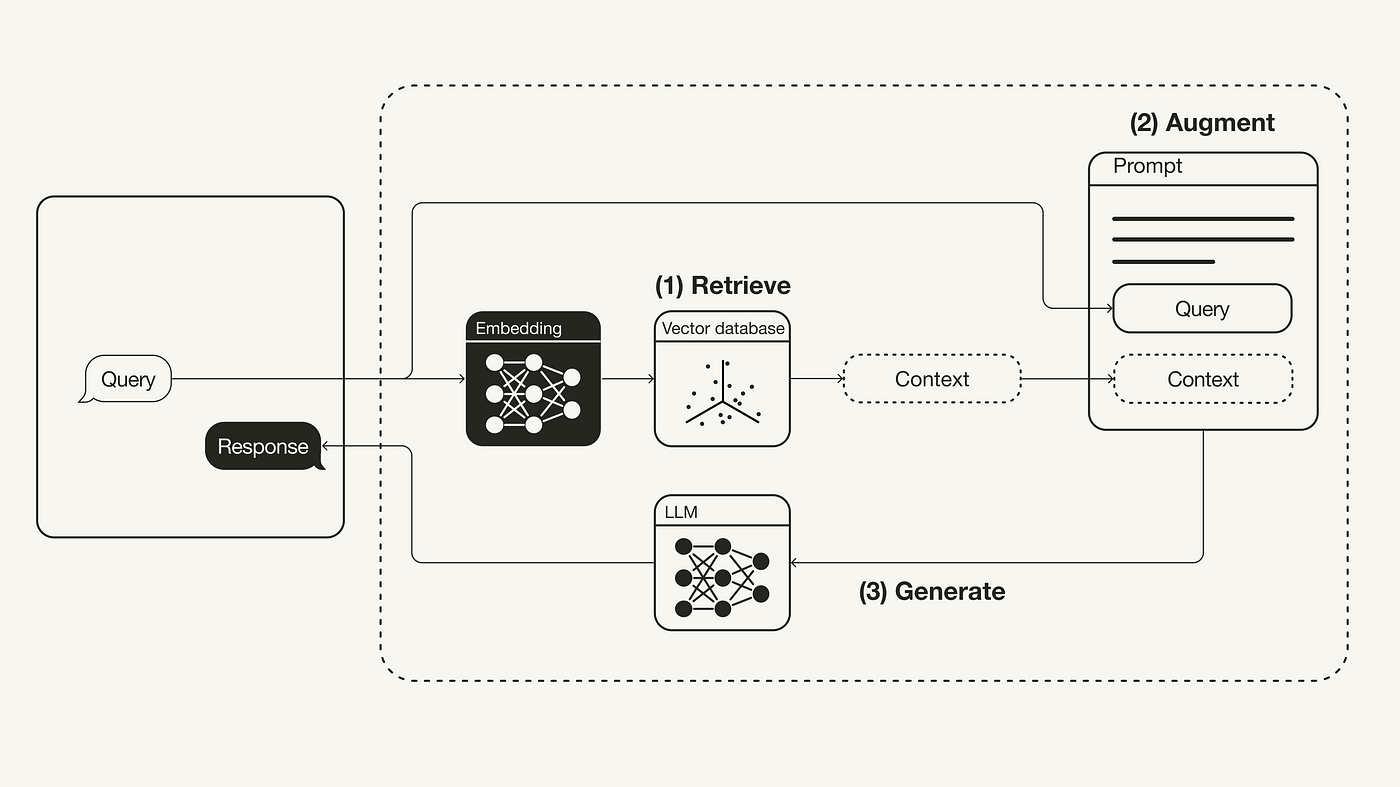
\includegraphics[scale=0.3]{figures/Rag.png}
	\caption{ Retrieval Augmented Generation }
\end{figure}

\newpage

Retrieval-Augmented Generation is particularly beneficial for knowledge-intensive tasks where accurate and comprehensive knowledge retrieval is crucial. Some notable applications include:



\begin{itemize}
    \item \textbf{Question Answering:} Enhancing the ability to answer complex questions by leveraging a broader range of external knowledge.
    \item \textbf{Dialogue Systems:} Improving the responses of chatbots by integrating real-time information retrieval.
    \item \textbf{Summarization:} Generating concise summaries enriched with up-to-date information from external sources.
    \item \textbf{Content Creation:} Facilitating the creation of informative and well-researched content by incorporating diverse perspectives and facts.
\end{itemize}


\hfill \break
The advantages of Retrieval-Augmented Generation include:
\begin{itemize}
    \item \textit{Accuracy:} Integrating external knowledge sources helps in providing more accurate and relevant responses.
    \item \textit{Coverage:} It expands the scope of information that can be accessed beyond what is inherently encoded in the model.
    \item \textit{Flexibility:} The approach is flexible and adaptable to different domains and tasks by selecting appropriate retrieval sources.
\end{itemize}

\newpage
\hfill \break
However, there are challenges associated with RAG:
\begin{itemize}
    \item \textit{Efficiency:} Retrieval can be computationally expensive, especially with large knowledge bases.
    \item \textit{Integration Complexity:} Harmonizing retrieved knowledge with the generation model output without losing coherence can be challenging.
    \item \textit{Evaluation:} Assessing the quality of generated outputs that depend on retrieved knowledge poses evaluation challenges.
\end{itemize}

To understand the technical architecture of RAG models, consider the following components:
\begin{itemize}
    \item \textbf{Retriever Model:}
    \begin{itemize}
        \item \textit{Indexing:} The retriever model first indexes a large corpus of documents or knowledge base.
        \item \textit{Query Encoding:} When a query is input, the retriever encodes it into a dense vector representation.
        \item \textit{Similarity Search:} The encoded query is compared with the indexed document vectors to retrieve the most relevant documents.
    \end{itemize}

    \item \textbf{Generator Model:}
    \begin{itemize}
        \item \textit{Contextual Embeddings:} The retrieved documents are transformed into contextual embeddings, which are combined with the query embeddings.
        \item \textit{Attention Mechanisms:} Advanced attention mechanisms allow the generator to attend to relevant parts of the retrieved documents while generating the response.
        \item \textit{Sequence Generation:} Using transformer-based architectures, the generator produces the output text, conditioned on the combined context of the query and retrieved documents.
    \end{itemize}
\end{itemize}

\newpage

An example workflow for a knowledge-intensive task, such as answering a detailed historical question, might involve:
\begin{itemize}
    \item \textbf{Input Query:} "What were the key factors that led to the fall of the Roman Empire?"
    \item \textbf{Retrieval Phase:}
    \begin{itemize}
        \item \textit{Query Encoding:} Encode the query using a model like BERT.
        \item \textit{Similarity Search:} Retrieve relevant passages from a historical database or Wikipedia.
        \item \textit{Selected Passages:} Identify key documents discussing economic troubles, military losses, and political corruption.
    \end{itemize}
    \item \textbf{Integration Phase:}
    \begin{itemize}
        \item \textit{Contextual Integration:} Integrate the retrieved passages into the generation context.
    \end{itemize}
    \item \textbf{Generation Phase:}
    \begin{itemize}
        \item \textit{Response Generation:} Generate a comprehensive answer that weaves together information from the retrieved passages, highlighting economic, military, and political factors.
    \end{itemize}
\end{itemize}

\begin{itemize}
    \item \textbf{Scalability:} Developing more efficient retrieval algorithms and data structures to handle ever-larger knowledge bases.
    \item \textbf{Personalization:} Tailoring retrieval and generation processes to individual user preferences and contexts.
    \item \textbf{Multimodal Retrieval:} Extending RAG to handle multimodal data, incorporating text, images, and other media types.
    \item \textbf{Evaluation Metrics:} Creating better evaluation metrics to assess the factual accuracy, relevance, and coherence of generated content.
\end{itemize}

\newpage
Practical applications and case studies of RAG include:
\begin{itemize}
    \item \textbf{Chat-bot support:}
    \begin{itemize}
        \item \textit{Scenario:} A support chatbot for a tech company.
        \item \textit{Implementation:} Integrate a knowledge base of product manuals and troubleshooting guides. Use RAG to retrieve relevant sections and generate tailored responses to customer queries.
    \end{itemize}
    \item \textbf{Educational Tools:}
    \begin{itemize}
        \item \textit{Scenario:} An interactive learning platform for history students.
        \item \textit{Implementation:} Access a large repository of historical texts. RAG retrieves pertinent excerpts and generates explanatory content or answers to student questions.
    \end{itemize}
    
\end{itemize}

\hfill \break
Here is the link to the RAG Pipline repository: \url{https://github.com/Sh-31/NeuraLearn-ML-Server-QG-RAG-Pipeline}

\newpage

\section{Training and Evaluation}
\subsection{Question Generation}

There was a several implementation for question generation model
I will present the final model and do comparison of variance architecture and number of parameter in evaluation section.

\hfill \break
\textbf{Training Arguments:}
\begin{figure}[h!]
	\centering
	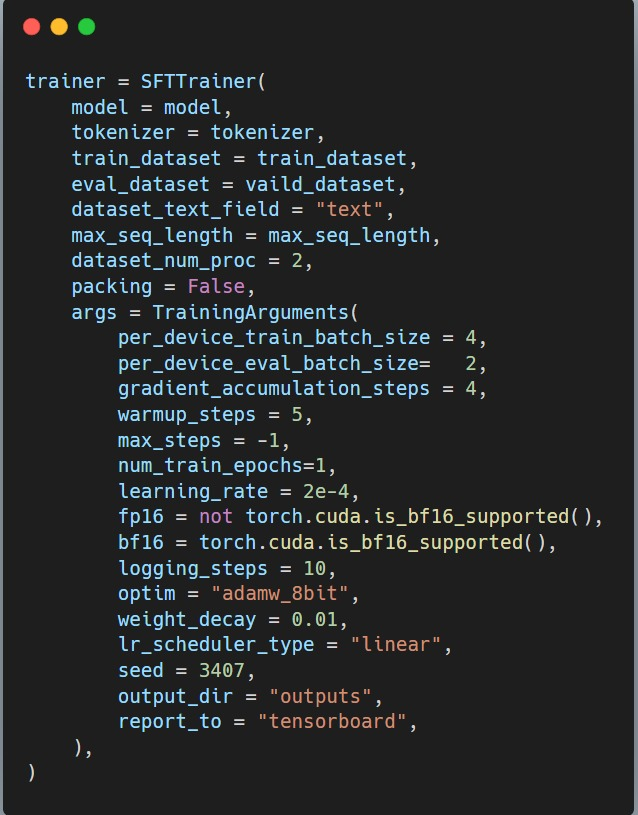
\includegraphics[scale=0.6]{figures/qg_argrs.png}
	\caption{ Question Generation Training Arguments }
\end{figure}

\newpage

\begin{figure}[h!]
	\centering
	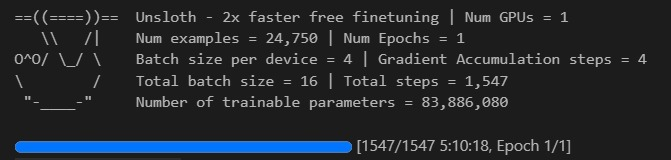
\includegraphics[scale=0.6]{figures/qg_info.jpeg}
	\caption{ Number of parameter  }
\end{figure}


\hfill \break
\textbf{Training loss vs steps :}

\begin{figure}[h!]
	\centering
	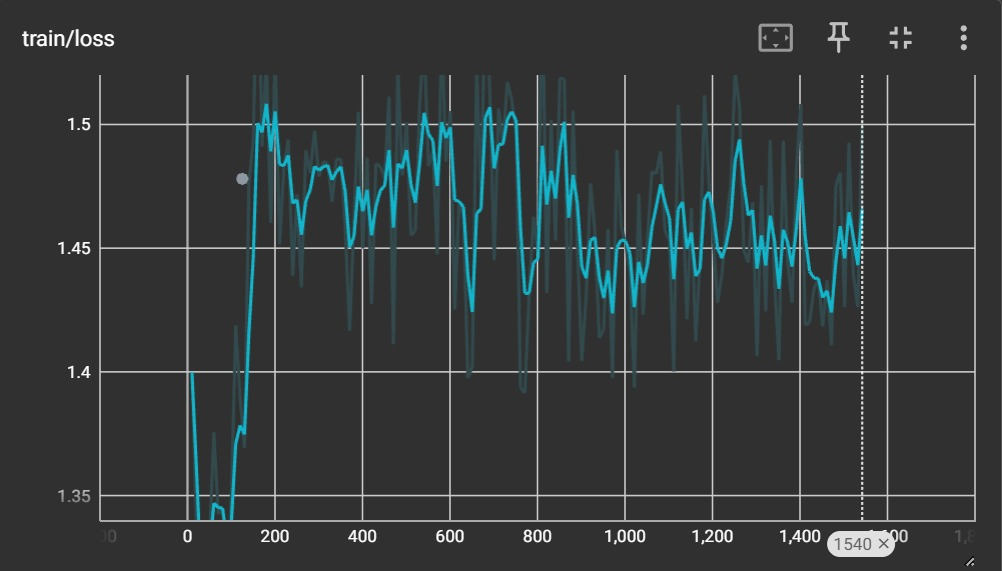
\includegraphics[scale=0.4]{figures/qg_train_loss.jpeg}
	\caption{ Question Generation Training Loss vs Steps }
\end{figure}

\begin{figure}[h!]
	\centering
	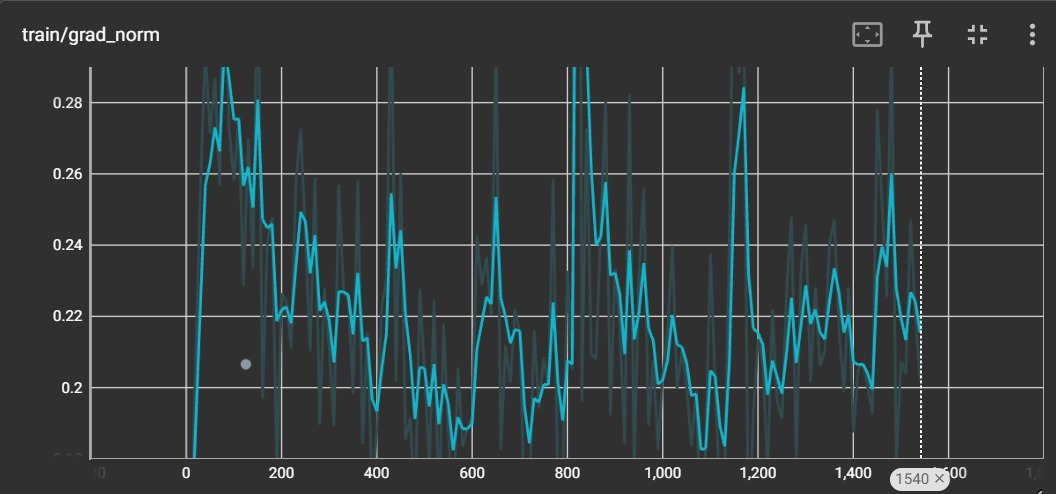
\includegraphics[scale=0.4]{figures/grad_norm.jpeg}
	\caption{ Question Generation Training grad norm vs Steps }
\end{figure}
\newpage

\hfill \break
\textbf{Metrics evaluation:} 

\hfill \break
\textbf{How to evaluation:}

\hfill \break
Based on "Are Large Language Models Fit For Guided Reading?" Paper \cite{ochieng2023large} looks at the ability of large language models to participate in educational
guided reading. We specifically, evaluate their ability to generate meaningful
questions from the input text, generate diverse questions.

It's suggest use ROUGE-L and BERTScore as evaluation metric.

\begin{figure}[h!]
	\centering
	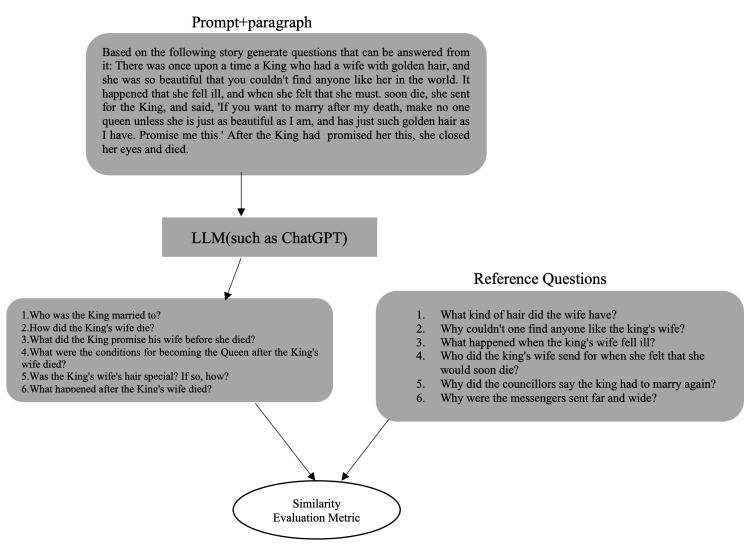
\includegraphics[scale=0.5]{figures/generate questions from a given text input.jpeg}
	\caption{ Prompting LLM to generate questions from a given text input  }
\end{figure}

\begin{figure}[h!]
	\centering
	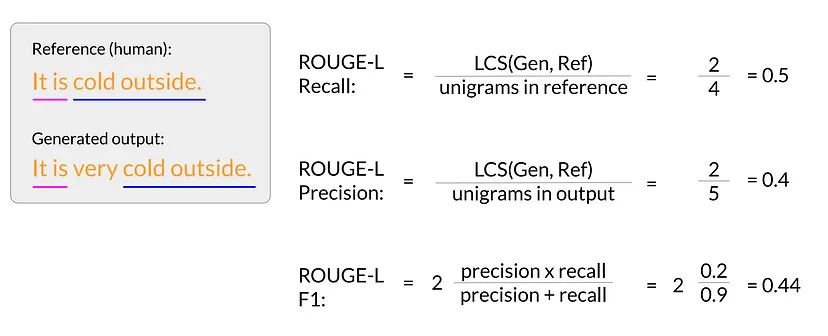
\includegraphics[scale=0.5]{figures/ROUGE-L.png}
	\caption{ROUGE-L}
\end{figure}

\newpage
\begin{table}[h!]
    \centering
    \begin{tabular}{|>{\raggedright\arraybackslash}p{5cm}|>{\centering\arraybackslash}p{2cm}|>{\centering\arraybackslash}p{2cm}|>{\centering\arraybackslash}p{2cm}|>
    {\centering\arraybackslash}p{2cm}|>{\centering\arraybackslash}p{2cm}|}
        \hline
        \textbf{Model} & \textbf{Adapter Rank} & \textbf{ROUGE-1} & \textbf{ROUGE-2} & \textbf{ROUGE-L} & \textbf{ROUGE-Lsum} \\
        \hline
        LLaMA-3 8B & 32 & 0.4024 & 0.1956 & 0.3790 & 0.3381 \\
        \hline
        LLaMA-3 8B & 16 & 0.3637 & 0.1025 & 0.2997 & 0.3546 \\
        \hline
        Gemma 2B & 32 & 0.3642 & 0.0998 & 0.3068 & 0.3536 \\
        \hline
        Gemma 2B & 16 & 0.3003 & 0.2111 & 0.2368 & 0.3234 \\
        \hline
    \end{tabular}
    \caption{Comparison of ROUGE scores for different models and adapter ranks}
    \label{tab:rouge_scores}
\end{table}


\hfill \break
\textbf{What's a good ROUGE score?:}

\hfill \break
A good ROUGE score varies by task and metric. ROUGE-1 scores are excellent around 0.5, with scores above 0.5 considered good and 0.4 to 0.5 moderate. For ROUGE-2, scores above 0.4 are good, and 0.2 to 0.4 are moderate.

\hfill \break
ROUGE-L scores are good around 0.4 and low at 0.3 to 0.4. While ROUGE scores are useful, they don't account for semantic or syntactic quality and should be complemented with other metrics and human evaluation for a complete assessment.

\hfill \break

Important Note: we didn't use any type of beam search algorithm to enhance the result because of competition power resource is limited.
\begin{figure}[h!]
	\centering
	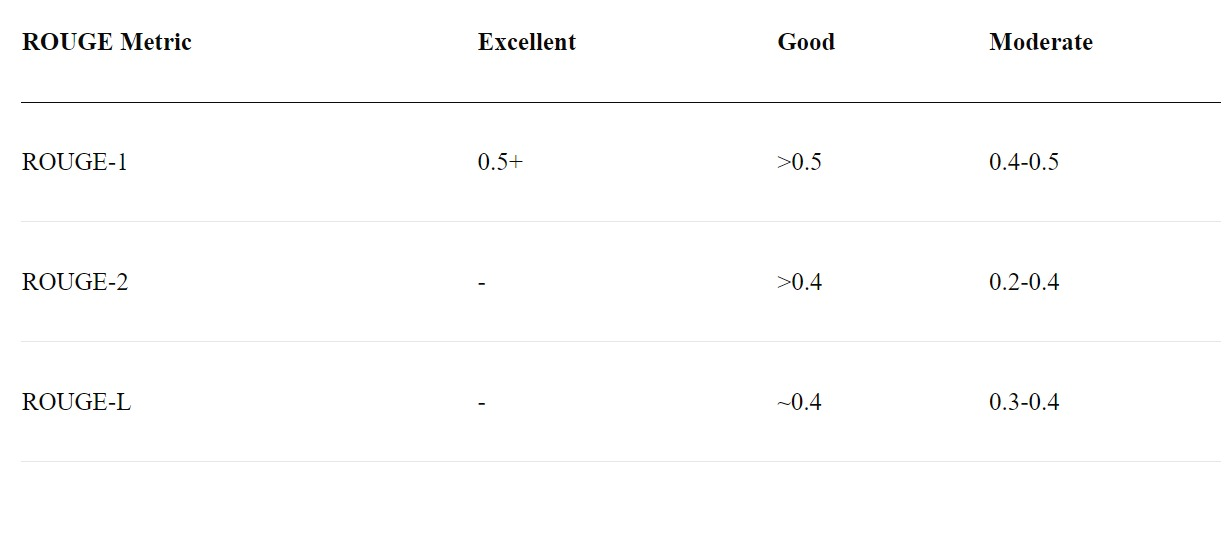
\includegraphics[scale=0.4]{figures/What's a good ROUGE score.png}
	\caption{ What's a good ROUGE score? }
\end{figure}

\newpage
\begin{figure}[h!]
	\centering
	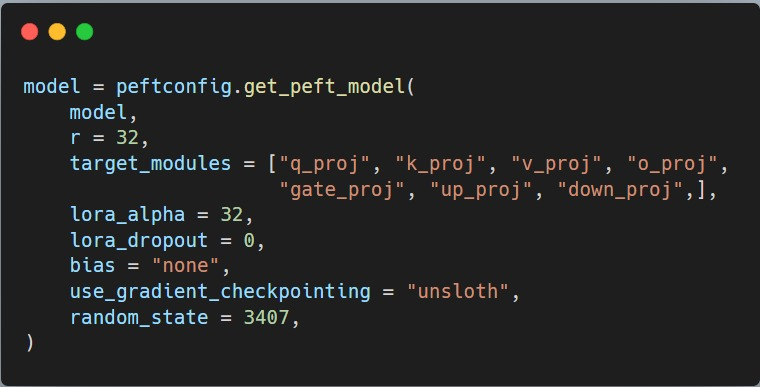
\includegraphics[scale=0.6]{figures/Adapter config rank 32.jpeg}
	\caption{ Adapter config rank 32 }
\end{figure}



\begin{figure}[h!]
	\centering
	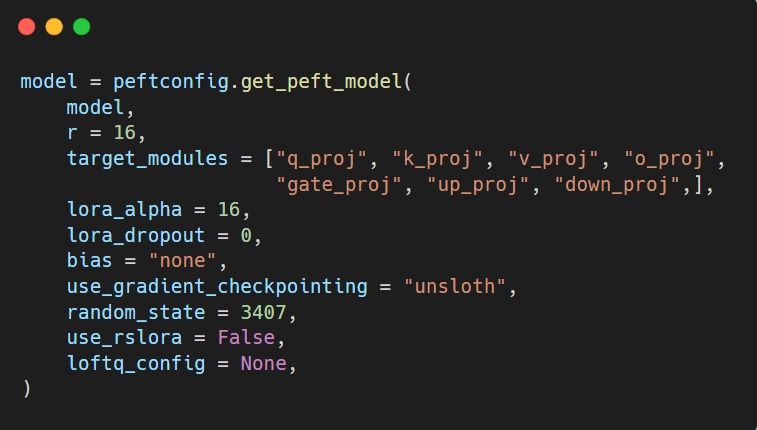
\includegraphics[scale=0.6]{figures/Adapter config rank 16.jpeg}
	\caption{ Adapter config rank 16 }
\end{figure}

\hfill \break
Here is the link to the model repository: \url{https://huggingface.co/shredder-31/Llamma-3_QG_V.3.0}

\newpage
\subsection{Text summarization }

Our text summarization model is based of \cite{beltagy2020longformer} longformer is a variant of the transformer architecture designed to handle long-range dependencies more effectively than traditional Transformers, which typically have a quadratic dependency on the sequence length due to their self-attention mechanism. 

\hfill \break
\hfill \break
\textbf{Training Arguments:}


\begin{figure}[h!]
	\centering
	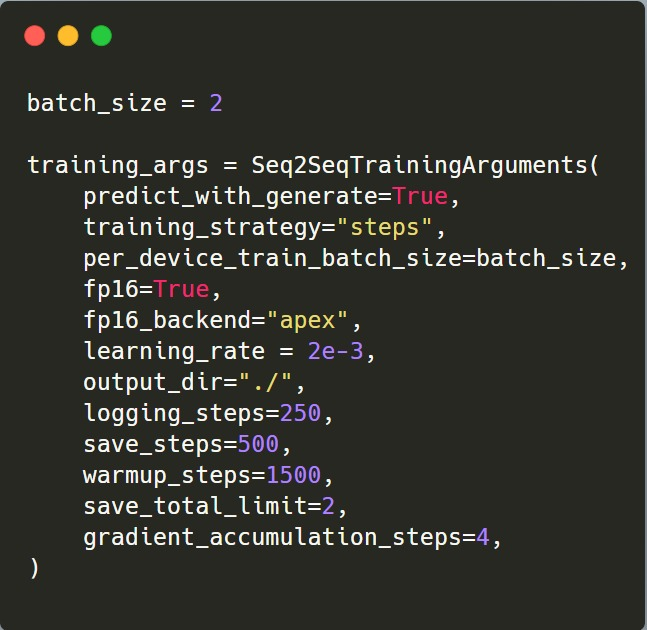
\includegraphics[scale=0.6]{figures/SummarizationTraining Arguments.png}
	\caption{ Summarizing Training Arguments }
\end{figure}


\newpage

\hfill \break
\textbf{Training loss vs steps :}

\begin{figure}[h!]
	\centering
	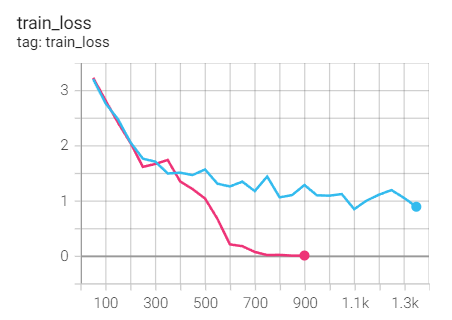
\includegraphics[scale=0.8]{figures/Summarization Training Loss vs Steps.png.png}
	\caption{ Summarizing Training Loss vs Steps }
\end{figure}

\hfill \break
\textbf{Val loss vs steps :}

\begin{figure}[h!]
	\centering
	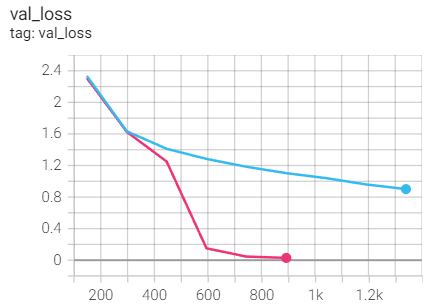
\includegraphics[scale=0.8]{figures/Summarization Val Loss vs Steps.png.png}
	\caption{ Summarizing Training Loss vs Steps }
\end{figure}

\newpage
\hfill \break
\textbf{Metrics evaluation:} 

\begin{table}[h!]
    \centering
    \begin{tabular}{|c|c|}
        \hline
        \textbf{Metric} & \textbf{Value} \\
        \hline
        ROUGE-1 & 0.32\\
        \hline
        ROUGE-2 & 0.6 \\
        \hline
        ROUGE-L & 0.16 \\
        \hline
        ROUGE-LSUM & 0.29 \\
        \hline
    \end{tabular}
    \caption{Performance Metrics on booksum benchmark}
    \label{tab:performance_metrics}
\end{table}

\begin{table}[h!]
    \centering
    \begin{tabular}{|c|c|}
        \hline
        \textbf{Metric} & \textbf{Value} \\
        \hline
        ROUGE-1 & 0.30 \\
        \hline
        ROUGE-2 & 0.13 \\
        \hline
        ROUGE-L & 0.19 \\
        \hline
        ROUGE-LSUM & 0.28 \\
        \hline
    \end{tabular}
    \caption{Performance Metrics on samsum dataset}
    \label{tab:performance_metrics}
\end{table}


\begin{table}[h!]
    \centering
    \begin{tabular}{|c|c|}
        \hline
        \textbf{Metric} & \textbf{Value} \\
        \hline
        ROUGE-1 & 0.36 \\
        \hline
        ROUGE-2 & 0.15 \\
        \hline
        ROUGE-L & 0.23 \\
        \hline
        ROUGE-LSUM & 0.30 \\
        \hline
    \end{tabular}
    \caption{Performance Metrics on billsum dataset}
    \label{tab:performance_metrics}
\end{table}

\hfill \break
Here is the link to the model repository: \url{https://huggingface.co/shredder-31/Summarization_Model_led_base_book_summary}

\newpage
\section{Literature review}
\begin{figure}[h!]
\begin{center}
	\centering
        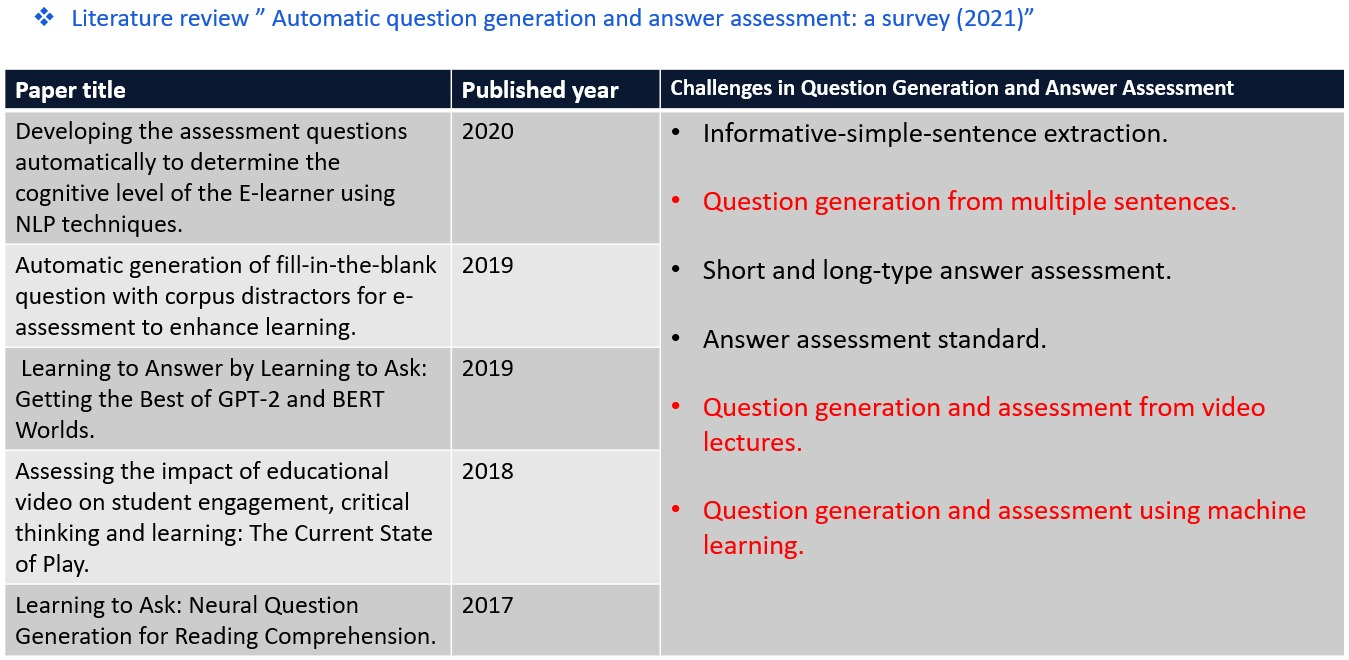
\includegraphics[width=1.2\textwidth]{figures/Literature review.png}
	\caption{Literature review ”Automatic question generation and answer assessment: a survey (2021)”}
\end{center}
\end{figure}




